% Source: graduate-coursework/Sp26/CSCE763/Course_Assignments/Project/project_proposal.tex

\documentclass[border=4pt]{standalone}
\usepackage{amsmath}
\usepackage{amssymb}
\usepackage{graphicx}
\usepackage{tikz}
\usepackage{xcolor}
\usetikzlibrary{positioning, arrows.meta, calc, fit, backgrounds, decorations.pathreplacing}

\definecolor{USC_Garnet}{HTML}{73000A}
\definecolor{USC_Black10}{HTML}{ECECEC}
\definecolor{USC_Black70}{HTML}{5C5C5C}
\definecolor{USC_Congaree}{HTML}{1F414D}

\begin{document}
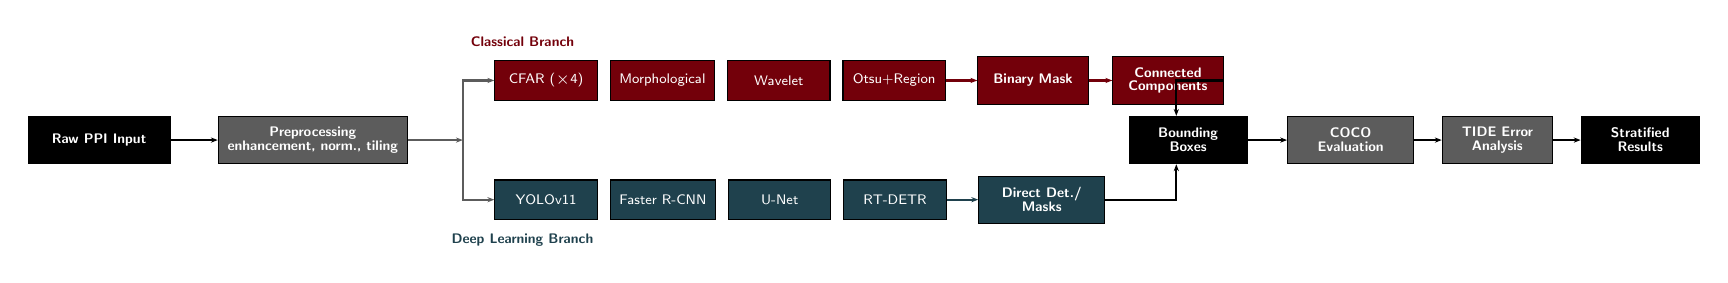
\begin{tikzpicture}[
  every node/.style={font=\sffamily\scriptsize},
  block/.style={draw, fill=#1, text=white, minimum height=0.6cm, minimum width=1.5cm, font=\sffamily\tiny\bfseries, align=center},
  block/.default={USC_Black70},
  sblock/.style={draw, fill=#1, text=white, minimum height=0.5cm, minimum width=1.3cm, font=\sffamily\tiny, align=center},
  sblock/.default={USC_Garnet},
  arr/.style={-{Stealth[length=2.5pt]}, thick},
  darr/.style={-{Stealth[length=2.5pt]}, thick, USC_Black70},
]
  % Input
  \node[block=black, minimum width=1.8cm] (input) {Raw PPI Input};

  % Preprocessing
  \node[block=USC_Black70, right=0.6cm of input, minimum width=2.2cm] (pre) {Preprocessing\\[-1pt]\tiny enhancement, norm., tiling};

  % Branch split point
  \coordinate[right=0.7cm of pre] (split);

  % Classical branch
  \node[sblock=USC_Garnet, above right=0.5cm and 0.4cm of split] (cfar) {CFAR ($\times$4)};
  \node[sblock=USC_Garnet, right=0.15cm of cfar] (morphm) {Morphological};
  \node[sblock=USC_Garnet, right=0.15cm of morphm] (wavem) {Wavelet};
  \node[sblock=USC_Garnet, right=0.15cm of wavem] (otsum) {Otsu+Region};

  % Classical intermediate
  \node[block=USC_Garnet, right=0.4cm of otsum, minimum width=1.4cm] (bmask) {Binary Mask};
  \node[block=USC_Garnet, right=0.3cm of bmask, minimum width=1.4cm] (cc) {Connected\\[-1pt]Components};

  % Deep learning branch
  \node[sblock=USC_Congaree, below right=0.5cm and 0.4cm of split] (yolo) {YOLOv11};
  \node[sblock=USC_Congaree, right=0.15cm of yolo] (frcnn) {Faster R-CNN};
  \node[sblock=USC_Congaree, right=0.15cm of frcnn] (unet) {U-Net};
  \node[sblock=USC_Congaree, right=0.15cm of unet] (rtdetr) {RT-DETR};

  % DL intermediate
  \node[block=USC_Congaree, right=0.4cm of rtdetr, minimum width=1.6cm] (direct) {Direct Det./\\[-1pt]Masks};

  % Bounding boxes (merge point)
  \coordinate[right=0.3cm of cc] (mergeTop);
  \coordinate[right=0.3cm of direct] (mergeBot);
  \coordinate (mergeC) at ($(mergeTop)!0.5!(mergeBot)$);
  \node[block=black, minimum width=1.5cm] at (mergeC) (bbox) {Bounding\\[-1pt]Boxes};

  % Evaluation
  \node[block=USC_Black70, right=0.5cm of bbox, minimum width=1.6cm] (coco) {COCO\\[-1pt]Evaluation};
  \node[block=USC_Black70, right=0.35cm of coco, minimum width=1.4cm] (tide) {TIDE Error\\[-1pt]Analysis};
  \node[block=black, right=0.35cm of tide, minimum width=1.5cm] (results) {Stratified\\[-1pt]Results};

  % Arrows
  \draw[arr] (input) -- (pre);
  \draw[darr] (pre) -- (split);
  % Split to branches
  \draw[darr] (split) |- (cfar);
  \draw[darr] (split) |- (yolo);
  % Classical chain
  \draw[arr, USC_Garnet] (otsum) -- (bmask);
  \draw[arr, USC_Garnet] (bmask) -- (cc);
  % DL chain
  \draw[arr, USC_Congaree] (rtdetr) -- (direct);
  % To bounding boxes
  \draw[arr] (cc.east) -| ([xshift=-0.15cm]bbox.north);
  \draw[arr] (direct.east) -| ([xshift=-0.15cm]bbox.south);
  % Evaluation chain
  \draw[arr] (bbox) -- (coco);
  \draw[arr] (coco) -- (tide);
  \draw[arr] (tide) -- (results);

  % Branch labels
  \node[USC_Garnet, font=\sffamily\tiny\bfseries, above=0.05cm of cfar, xshift=-0.3cm] {Classical Branch};
  \node[USC_Congaree, font=\sffamily\tiny\bfseries, below=0.05cm of yolo, xshift=-0.3cm] {Deep Learning Branch};
\end{tikzpicture}
\end{document}
